\documentclass[handout]{beamer}

\usepackage{Vor2018glærur}

\title{Tölvunarfræði 2}
\subtitle{Vika 3}

\begin{document}

\begin{frame}
\titlepage
\end{frame}

\section{Meira um vector}

\begin{frame}{\texttt{vector}}
\begin{itemize}
 \item Við höfum notað \texttt{std::vector} og líkt gagnagerðinni við fylki í C-stíl
 \begin{itemize}
  \item Getur verið svipað í notkun, en virkar á töluvert frábrugðinn máta
 \end{itemize}
 \item \texttt{vector} er klasi sem sér um ýmislegt minnisbókhald fyrir okkur
 \begin{itemize}
  \item Venjulega eru gögn \texttt{vector} tilviks geymd í kös þó að hluturinn sjálfur þurfi ekki að vera þar
  \item Sér um eigin ruslasöfnun
  \item Sér (oftast) um að sér sé skilað á skilvirkan hátt (lesefnisuppástunga: \emph{move semantics})
 \end{itemize}
 \item Við gætum gert svipaðan klasa! (\href{https://gcc.gnu.org/onlinedocs/libstdc++/latest-doxygen/a01523_source.html}{stl\_vector.h} í GCC)
\end{itemize}
\end{frame}

\begin{frame}{Bak við tjöldin}
\begin{itemize}
 \item \texttt{vector} er ætlað að vera ``kvikt fylki'' sem getur höndlað mörg notkunartilvik, en bak við tjöldin þurfa samt að fara fram minnisúthlutanir
 \item Endurteknar minnisúthlutanir geta tekið mikinn tíma 
 \item Lausnin sem \texttt{vector} fer - forúthlutun
 \begin{itemize}
  \item Skoðum \texttt{sizecapacity.cpp}
 \end{itemize}
\end{itemize}
\end{frame}

\section{Fleiri gagnagerðir}

\subsection{Strengir}

\begin{frame}{\texttt{string}}
\begin{itemize}
 \item Við þurfum oft að vinna með texta, til þess er hægt að nota gagnagerðina \texttt{char}
 \begin{itemize}
  \item Til að fá strengi með \texttt{char} þarf að nota fylki af táknum
  \item Fylki af táknum eru ekki jafn meðfærileg og við búumst við af strengjum úr öðrum forritunarmálum 
 \end{itemize}
 \item Líkt og \texttt{std::vector} gerir almenna fylkjavinnslu þægilegri gerir \texttt{std::string} sérhæfða strengjavinnslu þægilegri
\end{itemize}
\end{frame}

\begin{frame}{Kostir \texttt{string}}
\begin{itemize}
 \item Líkt og \texttt{vector} sér \texttt{string} um sína eigin minnisstjórnun
 \begin{itemize}
  \item Í C++11, gert mjög vel
 \end{itemize}
 \item Innbyggðir virkjar
 \item Innbyggð föll
\end{itemize}
\end{frame}

\begin{frame}{Hvað er hægt að gera við \texttt{string}?}
\cppfile[firstline=7, lastline=11, label=stringtricks.cpp]{Code/w3/stringtricks.cpp}
\cppfile[firstline=15, lastline=20, label=stringtricks.cpp]{Code/w3/stringtricks.cpp}
\end{frame}

\begin{frame}{Hvað er hægt að gera við \texttt{string}?}
\cppfile[firstline=24, lastline=27, label=stringtricks.cpp]{Code/w3/stringtricks.cpp}
\cppfile[firstline=31, lastline=34, label=stringtricks.cpp]{Code/w3/stringtricks.cpp}
\end{frame}

\subsection{Mengi}

\begin{frame}{Mengi}
\texttt{std::set} skilgreinir mengi staka, án endurtekninga. \texttt{std::multiset} skilgreinir safn staka, með endurtekningum.

\begin{center}
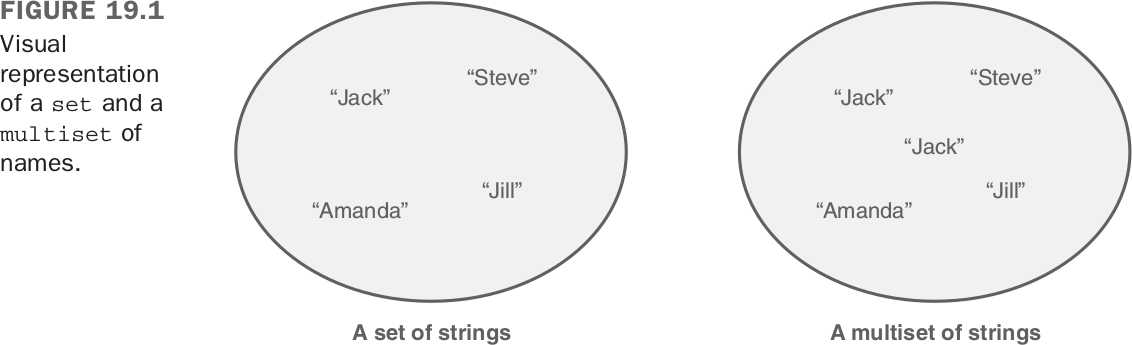
\includegraphics[width=\textwidth]{set-multiset}
\end{center}


Ólíkt þeim mengjum sem við þekkjum úr stærðfræði eru þessi mengi röðuð!
\end{frame}

\begin{frame}{Röðuð og óröðuð mengi}
\begin{itemize}
 \item \texttt{set} og \texttt{multiset} eru skilgreind í \texttt{<set>}
 \begin{itemize}
  \item Til að hægt sé að setja klasa sem við höfum skrifað í þessi mengi þurfa þeir að vera samanberanlegir
  \item Fjölbinding fyrir < virkjann!
 \end{itemize}
 \item Nýtt í C++11: \texttt{unordered\_set} og \texttt{unordered\_multiset} eru skilgreind í \texttt{<unordered\_set>}
 \begin{itemize}
  \item Þurfum að útfæra \href{http://en.cppreference.com/w/cpp/utility/hash}{hakkafall} fyrir klasana okkar til að hægt sé að geyma þá í óröðuðum mengjum
 \end{itemize}
 \item Aðgerðir á mengin hafa mismundandi tímaflækjur
 \item Munum kynnast þessum betur síðar
\end{itemize}
\end{frame}

\subsection{Varpanir}

\begin{frame}{Varpanir}
\begin{columns}
\column{0.4\textwidth}
\begin{itemize}
 \item \texttt{std::map} og \texttt{std::multimap} tengja saman lykla (e. \emph{keys}) og gildi (e. \emph{values})
 \item Skoðum \texttt{multimapexample.cpp}
\end{itemize}
\column{0.6\textwidth}
\begin{center}
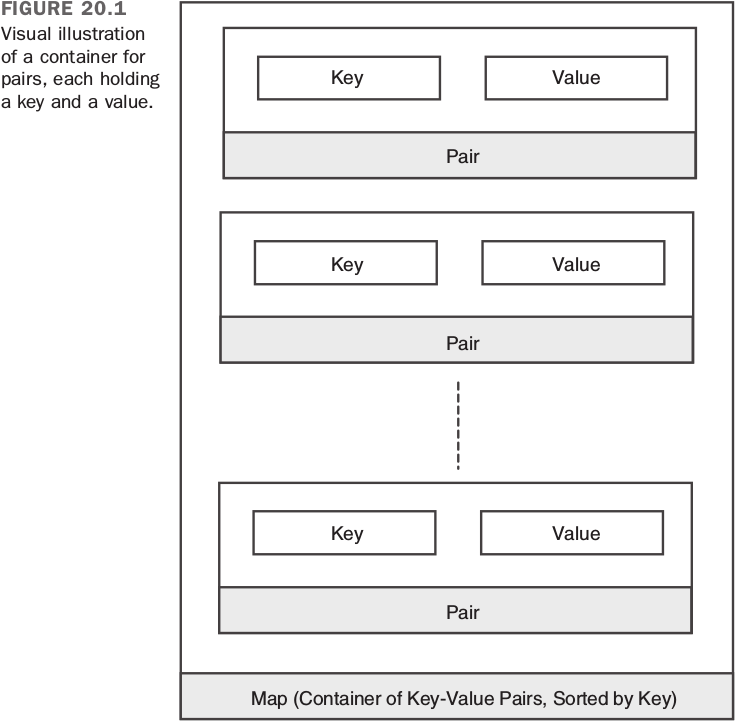
\includegraphics[width=\linewidth]{map}
\end{center}
\end{columns}
\end{frame}

\section{STL hjálpartæki}

\begin{frame}{Ítrarar}
\begin{itemize}
 \item Ítrarar (e. \emph{iterators}) eru að sumu leyti svipaðir bendum, notaðir til að vísa til sérstakra staka
 \item Dæmi:
 \begin{itemize}
  \item Föllin \texttt{begin()} og \texttt{end()} skila ítrurum sem vísa til fyrsta/síðasta staks í STL gagnagerð
 \end{itemize}
 \item Þykja nútímaleg leið til að vísa á stök
 \begin{itemize}
  \item Svipuð fyrirbrigði koma fyrir í mörgum nýrri forritunarmálum
 \end{itemize}
 \item Sjá töflu: \url{http://www.cplusplus.com/reference/iterator/}
\end{itemize}

\end{frame}


\begin{frame}{Reiknirit}
\begin{itemize}
 \item Gagnagerðir í STL eru hannaðar til að virka með ýmsum hjálparföllum, m.a.
 \begin{itemize}
  \item \texttt{reverse} - snýr við röðun á safninu
  \item \texttt{find} - finnur ákveðið stak í safninu
  \item \texttt{transform} - beitir gefnu falli á safnið
 \end{itemize}
 \item Til að nota föllin þarf \texttt{algorithms} hausinn
\end{itemize}
\end{frame}

\section{Meira um C++}

\subsection{Hausar og margar skrár}

\begin{frame}{Hausar og margar skrár}
\begin{itemize}
 \item Við getum látið C++ forrit teygja sig yfir margar skrár
 \item Hægt að þýða margar í einu: \texttt{\$ g++ skra1.cpp skra2.cpp}
 \begin{itemize}
  \item Setjum skilgreiningar í \texttt{.h} skrár
  \item Vísum í þær með \texttt{\#include}
  \item GCC þekkir staðsetningar innbyggðra hausa eins og \texttt{iostream}
  \item Þurfum ekki að þýða allar skrárnar ef sumar eru óbreyttar!
 \end{itemize}
 \item Skoðum \texttt{myclass.cpp}, \texttt{myclass.h} og \texttt{runmyclass.cpp}
\end{itemize}
\end{frame}

\subsection{Optimization levels}

\begin{frame}{Hverju skilar þýðandinn?}
\begin{itemize}
 \item C++ þýðandi getur þýtt kóða á mismunandi hátt!
 \item Mikilvægt dæmi: Bestunarstillingar GCC
 \begin{itemize}
  \item Hægt er að ákveða hversu hart þýðandinn á að ganga fram við að búa til besta mögulega kóða
  \item Sjálfgefið er að þýðingin sé hröð, ekki að hún skili hröðum kóða
  \item \href{https://gcc.gnu.org/onlinedocs/gcc/Optimize-Options.html}{GCC Optimize Options}
 \end{itemize}
 \item Sjá mismun: \href{http://godbolt.org/}{Godbolt}, \texttt{-S} valkostur GCC
\end{itemize}
\end{frame}

\begin{frame}{Skilvirk endurkvæmni í GCC}
\begin{columns}
\column{0.3\textwidth}
\begin{center}

\includegraphics[width=\linewidth]{stack-overflow}
\end{center}
\column{0.7\textwidth}
\begin{itemize}
 \item Endurkvæm forrit geta falið í sér ansi mörg fallsköll
 \begin{itemize}
  \item Getur valdið vandamálum í C++ ef hlaðinn fær að vaxa\pause
 \end{itemize}
 \item GCC getur oft endurnýtt vakningafærsluna (e. \emph{stack frame} eða \emph{activation record}) ef við gefum þýðandanum rétta valkosti
 \begin{itemize}
  \item \texttt{-foptimize-sibling-calls} og fleiri
  \item Innifalið í \texttt{-O2}, \texttt{-O3} og \texttt{-Os}
 \end{itemize}
 \item Auðveldast er að endurnýta halaendurkvæm (e. \emph{tail recursive}) fallsköll
\end{itemize}
\end{columns}
\end{frame}

\begin{frame}{Halaendurkvæmni}
\cppfile[firstline=4, lastline=10, fontsize=\scriptsize, label=recursivesum.cpp]{Code/w3/recursivesum.cpp}
\cppfile[firstline=4, lastline=10, fontsize=\scriptsize, label=tailrecursivesum.cpp]{Code/w3/tailrecursivesum.cpp}
\end{frame}

\section{Lokaorð}

\begin{frame}{Takmörkun}
\begin{itemize}
 \item Við kunnum ekki allt sem hægt er að læra í tengslum við C++ eftir þessar þrjár vikur
 \item En við eigum að kunna nóg til að\ldots
 \begin{enumerate}
  \item Forrita það sem forrita þarf í þessu námskeiði
  \item Eiga auðvelt með að læra meira!
 \end{enumerate}
\end{itemize}
\end{frame}


\begin{frame}{Þessi glærupakki}
Tengill á fyrirlestraræfingu: \url{https://goo.gl/forms/BCwTFqSjyeFYCsc12}
\vspace{1cm}

Öll nafngreind forrit í þessum glærupakka, ásamt glærupakkanum sjálfum, má finna á  \href{https://github.com/Ernir/kennsluefni/tree/master/T2/Code/w3}{Github}.
\end{frame}


\begin{frame}{Næst}
Inngangur að ADTs, Java
\end{frame}


\end{document}
